\documentclass[11pt,letterpaper]{article}
\usepackage{lmodern}
\usepackage[left=1.05in,right=1.05in,top=0.88in,bottom=0.92in]{geometry}
\usepackage[utf8]{inputenc}
\usepackage{amsmath,amssymb,amsthm,mathtools,booktabs,array,tabularx,microtype,xcolor}
\usepackage{tikz}
\usetikzlibrary{arrows.meta,positioning}
\usepackage[numbers,sort&compress]{natbib}
\usepackage{xurl}
\usepackage[colorlinks=true,linkcolor=blue!65!black,citecolor=blue!65!black,urlcolor=blue!65!black]{hyperref}
\hypersetup{
  pdftitle={Zero-Error Shannon Capacity of the Seven-Cycle: Exact Physical Subchannel Obstructions, Non-Cartesian Clique-Cover Lifts, and Historical Context},
  pdfauthor={Rudra Tiwari},
  pdfsubject={Exact restricted-alphabet obstructions and non-Cartesian clique-cover lifts for C_7^5 and C_7^10}
}
\setlength{\parindent}{1.5em}
\setlength{\parskip}{0pt}
\setlength{\emergencystretch}{2em}
\setcounter{tocdepth}{2}
\newtheorem{theorem}{Theorem}[section]
\newtheorem{lemma}[theorem]{Lemma}
\newtheorem{proposition}[theorem]{Proposition}
\newtheorem{corollary}[theorem]{Corollary}
\theoremstyle{definition}
\newtheorem{definition}[theorem]{Definition}
\theoremstyle{remark}
\newtheorem{remark}[theorem]{Remark}
\newcommand{\ThetaCap}{\Theta}
\newcommand{\varthetaL}{\vartheta}
\newcommand{\R}{\mathbb{R}}
\newcommand{\Z}{\mathbb{Z}}

\begin{document}
\thispagestyle{empty}
\begin{center}
\vspace*{0.22in}
{\LARGE\bfseries Structural Obstructions for Zero-Error Codes\\[.14em] on Powers of the Seven-Cycle\par}
\vspace{0.20in}
{\large Exact subchannel bounds and non-Cartesian clique-cover lifts\par}
\vspace{0.24in}
{\normalsize\bfseries Rudra Tiwari\par}
\vspace{0.03in}
{\normalsize\itshape University of Delhi, New Delhi, India\\Inter-University Accelerator Centre (IUAC), New Delhi, India\par}
\vspace{0.10in}
{\small\href{https://orcid.org/0009-0004-8521-7627}{ORCID: 0009-0004-8521-7627}\quad|\quad\href{https://rtx09x.github.io/}{Website}\quad|\quad\href{https://github.com/Rtx09x}{GitHub}\quad|\quad\href{https://github.com/Rtx09x/Open-Research/tree/main/mathematics/seven-cycle-shannon-capacity}{Open-Research}\par}
\vspace{0.15in}
{\normalsize November 2026\par}
\end{center}
\vspace{0.16in}
\begin{abstract}
Determining the zero-error Shannon capacity $\ThetaCap(C_7) = \sup_{k \ge 1} \alpha(C_7^{\boxtimes k})^{1/k}$ of the seven-cycle remains one of the oldest open problems in information theory and combinatorics. We do \emph{not} settle $\alpha(C_7^{\boxtimes 5})$ or $\ThetaCap(C_7)$, and we do \emph{not} claim a current-best global lower bound: our historical 768,000-dimensional recursive bound $\ThetaCap(C_7) \ge 3.258832624232849476\dots$ has been superseded by a stronger reported construction of Leo Tang ($\approx 3.258838705444608\dots$). Instead, this paper establishes exact, solver-free, standard-library-verified \emph{structural obstruction certificates} directly on the true physical confusability graphs of $C_7^{\boxtimes 5}$ and $C_7^{\boxtimes 10}$ (without terminal-label abstractions or numerical SDP trust). On $C_7^{\boxtimes 5}$, starting from the Polak--Schrijver 367-word code $I_0$, the Buys--Polak--Zuiddam auxiliary set $X$, and the graph automorphism $T(a,b,c,d,e)=((2-b)\bmod 7, d, a, (2-c)\bmod 7, e)$, we prove: (i)~$\ThetaCap(C_7^{\boxtimes 5}[U_2]) = 367$ exactly for $U_2 = I_0 \cup X$ ($702$ words, partitioned into $32K_1 + 335K_2$); (ii)~$\ThetaCap(C_7^{\boxtimes 5}[U_3]) \le 363 + 2\sqrt{5} < 367.5$ (rate $< 3.25870377$) for $U_3 = U_2 \cup T(I_0)$ ($704$ words, partitioned into $32K_1 + 331K_2 + 2C_5$), strictly separating the Lov\'asz $\varthetaL$-ceiling from the exact fractional clique cover value $368$; and (iii)~an exact rational fractional clique cover of weight $369000000413/10^9$ on $U_4 = U_3 \cup T(X)$ ($1009$ words, $5394$ edges), isolating $\alpha(C_7^{\boxtimes 5}[U_4]) \ge 368$ as a concrete unscreened decision gate. On $C_7^{\boxtimes 10}$, adjoining the seven-rectangle 134,753-word code $Z$ of Itty--Rosin--Carstensen--Reichman to $P_{382}^2$ and $P_{392}^2$ via non-Cartesian clique-cover lifting proves $\ThetaCap(C_7^{\boxtimes 10}[W_{382}]) = 134753$ exactly and $\ThetaCap(C_7^{\boxtimes 10}[W_{392}]) \le 134849$ (forcing at least $244$ words outside $W_{392}$ for any code of size $\ge 135093$), plus five exact 5,505-edge saturated matchings into $Z$. The stated subchannel certificates are checked with Python's standard library.
\end{abstract}
\vspace{0.10in}
\noindent\textbf{Keywords:} Shannon capacity, seven-cycle, zero-error information theory, Lov\'asz theta function, clique-cover lifting, exact combinatorial certificates.
\clearpage
\tableofcontents
\clearpage

\section{Introduction, Historical Context, and Strict Scope}
Since Shannon~\cite{Shannon1956} defined the zero-error capacity $\ThetaCap(G) = \sup_{k \ge 1} \alpha(G^{\boxtimes k})^{1/k}$ and Lov\'asz~\cite{Lovasz1979} settled $\ThetaCap(C_5)=\sqrt{5}$, the seven-cycle $C_7$ has remained the smallest unresolved odd cycle. Polak and Schrijver~\cite{PolakSchrijver2019} constructed a 367-word independent set $I_0 \subset C_7^{\boxtimes 5}$ giving $\ThetaCap(C_7) \ge 367^{1/5} \approx 3.25782$, while recent recursive and heterogeneous-substitution constructions by Buys, Polak, and Zuiddam~\cite{BPZ2026}, Itty, Rosin, Carstensen, and Reichman~\cite{IRCR2026} (a 134,753-word seven-rectangle code $Z \subset C_7^{\boxtimes 10}$), and Tandon~\cite{Tandon2026} pushed the lower bound past $3.25883$.

\paragraph{Historical construction context and why we make no current-best claim.}
An earlier recursive construction gave $\ThetaCap(C_7) \ge 3.258832624232849476\dots$. Tang reports the stronger lower bound $3.258838705444608\dots$~\cite{TaoConstants9a}.

\paragraph{What this paper contributes.}
Rather than tuning parameters inside exhausted label abstractions, this paper delivers \emph{exact, solver-free, physical-graph obstruction theorems} on natural automorphism and fiber-closure subchannels of $C_7^{\boxtimes 5}$ and $C_7^{\boxtimes 10}$, identifying precisely which word pools are closed across all block lengths and isolating the exact remaining combinatorial gates. Throughout, we maintain a strict distinction between restricted-alphabet subchannel capacity $\ThetaCap(C_7^{\boxtimes m}[U])$ and unrestricted $\ThetaCap(C_7)$: \emph{no theorem here upper-bounds unrestricted $\ThetaCap(C_7)$}.

\section{Exact Original-Channel Subchannel Obstructions on $C_7^{\boxtimes 5}$}
Encode five-coordinate words $(a,b,c,d,e) \in \Z_7^5$ as little-endian base-7 integers in $[0,16806]$. Two words are \emph{physically confusable} ($u \sim v$) iff every coordinate difference modulo $7$ lies in $\{0,1,6\}$. Let $I_0$ denote the 367-word Polak--Schrijver code~\cite{PolakSchrijver2019} (independently reconstructed term-for-term from the 382-word circular seed and 40 extension words in \texttt{verify\_published\_367.py}), let $X$ denote the 367-word auxiliary set of Buys--Polak--Zuiddam~\cite{BPZ2026} (from Tandon's pinned \texttt{base\_c7.json}~\cite{Tandon2026}), and define the $C_7^{\boxtimes 5}$ automorphism
\[
  T(a,b,c,d,e) = \bigl((2-b)\bmod 7,\; d,\; a,\; (2-c)\bmod 7,\; e\bigr).
\]
Consider the nested physical alphabets $U_2 = I_0 \cup X$ ($|U_2|=702$), $U_3 = U_2 \cup T(I_0)$ ($|U_3|=704$), and $U_4 = U_3 \cup T(X)$ ($|U_4|=1009$).

\begin{theorem}[Exact All-Length Capacity of $U_2$]\label{thm:u2}
The induced physical confusability graph $H_2 = C_7^{\boxtimes 5}[U_2]$ partitions disjointly into $32$ singleton vertices ($I_0 \cap X$) and $335$ physically confusable pairs ($K_2$) matching $I_0 \setminus X$ to $X \setminus I_0$. Consequently, for every block length $k \ge 1$, $\alpha(C_7^{\boxtimes 5k}[U_2^k]) = 367^k$, and
\[
  \ThetaCap(C_7^{\boxtimes 5}[U_2]) = 367.
\]
\end{theorem}
\begin{proof}
The $367^k$ Cartesian products of the $367$ physical cliques ($32K_1 + 335K_2$) partition $U_2^k$ into confusable cliques, forcing $\alpha(C_7^{\boxtimes 5k}[U_2^k]) \le 367^k$, while $I_0^k$ attains $367^k$.
\end{proof}

\begin{theorem}[Exact $\varthetaL$-Ceiling on $U_3$ and Separation from Fractional Clique Cover]\label{thm:u3}
The set $T(I_0) \setminus (I_0 \cup X)$ consists of exactly two words $\{6494, 13358\}$. The $704$ words of $H_3 = C_7^{\boxtimes 5}[U_3]$ admit a disjoint vertex partition into $32$ singletons, $331$ physically confusable pairs, and two explicit confusability $5$-cycles:
\[
  (6494,\, 8888,\, 6773,\, 6828,\, 4092) \qquad \text{and} \qquad (13358,\, 13065,\, 11062,\, 10677,\, 13364).
\]
Hence, by additivity, monotonicity under edge deletion, and Lov\'asz's identity $\varthetaL(C_5)=\sqrt{5}$~\cite{Lovasz1979},
\begin{equation}\label{eq:u3-theta}
  \ThetaCap(C_7^{\boxtimes 5}[U_3]) \le \varthetaL(H_3) \le 32 + 331 + 2\sqrt{5} = 363 + 2\sqrt{5} \approx 367.472135955 < 367.5,
\end{equation}
yielding per-coordinate rate $< 3.2587037677 < 3.258841$ across all block lengths $k \ge 1$. Moreover, the exact fractional clique-cover number of $H_3$ is $\chi_f(\overline{H_3}) = 368$ (matching primal/dual certificates), demonstrating that fractional clique cover fails to exclude $368$ whereas the elementary $2C_5$ Lov\'asz $\varthetaL$-partition does.
\end{theorem}

\begin{theorem}[Four-Code Gate $U_4$ and Local Exchange Cross-Checks]\label{thm:u4}
The induced graph $H_4 = C_7^{\boxtimes 5}[U_4]$ has $1009$ vertices, $5394$ physical confusability edges, and $3698$ maximal cliques ($2674$ triangles, $1022$ pairs, $2$ singletons). An explicit rational fractional clique cover on $883$ weighted physical cliques (common denominator $10^9$) proves
\[
  \alpha(C_7^{\boxtimes 5k}[U_4^k]) \le \left(\frac{369000000413}{10^9}\right)^k \qquad \forall k \ge 1
\]
(original-coordinate rate $< 3.26140906$). This does \emph{not} screen out $368$ or the target $3.258841$; isolating $\alpha(H_4) \ge 368$ yields a concrete unscreened $1009$-variable decision problem (an optional SciPy/HiGHS MILP run reported infeasible in 5 branch-and-bound nodes, but without an exact UNSAT proof it is not asserted as a theorem). Separately, direct physical enumeration over all $568{,}119$ support envelopes of size $\le 4$ outside $I_0$ confirms that all $3{,}842$ candidate-rich envelopes partition into $\le 4$ physical cliques (reproducing and structurally refining the prior 18 July 2026 no-4-for-5/no-5-for-6 exchange certificates of Mergen~\cite{Mergen2026}), and among $20{,}509$ center-5 unions in $U_4$, zero admit $6$ eligible outsiders.
\end{theorem}

\begin{figure}[!htbp]
\centering
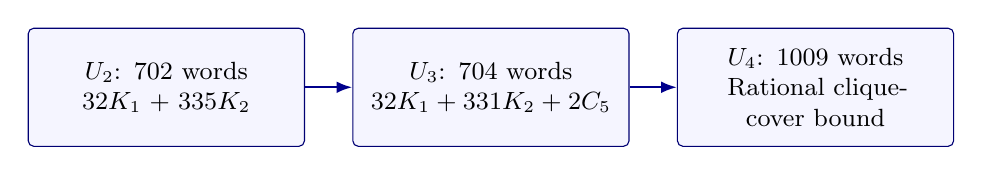
\begin{tikzpicture}[node distance=6mm,
 box/.style={draw=blue!45!black,rounded corners=2pt,fill=blue!4,align=center,text width=.27\linewidth,minimum height=15mm,font=\small},
 arrow/.style={-{Latex[length=2mm]},thick,blue!55!black}]
 \node[box] (u2) {$U_2$: $702$ words\\$32K_1+335K_2$};
 \node[box,right=of u2] (u3) {$U_3$: $704$ words\\$32K_1+331K_2+2C_5$};
 \node[box,right=of u3] (u4) {$U_4$: $1009$ words\\Rational clique-cover bound};
 \draw[arrow] (u2) -- (u3);
 \draw[arrow] (u3) -- (u4);
\end{tikzpicture}
\caption{Adding $T(I_0)$ to $U_2$ introduces two new words and creates the two five-cycle components in $U_3$. Adding $T(X)$ yields $U_4$, where the certificate uses a fractional cover.}
\end{figure}

\subsection{A separate finite-subgroup obstruction}
Any finite subgroup of $(\mathbb{R}/\mathbb{Z})^5$ with circular coordinate-max distance at least $2/7$ between distinct elements has at most $367$ elements. The same bound holds for a translate. Coordinatewise rounding maps a separated set injectively to an independent set in $C_7^{\boxtimes 5}$. The theta bound reduces the remaining group orders to $368$ through $401$. Characters of finite abelian groups reduce coverage of nonzero differences to an exact bit-mask search over cyclic and noncyclic types. The full reduction, search, and a separate implementation are supplied in the supplement. The bound concerns separated subgroup translates.

\section{Non-Cartesian Clique-Cover Lifting on $C_7^{\boxtimes 10}$}
Let $Z \subset C_7^{\boxtimes 10}$ be the seven-rectangle independent set of size $134{,}753$ constructed by Itty, Rosin, Carstensen, and Reichman~\cite{IRCR2026} from $I_0$, $X$, and the disjoint subsets $R, H, V$ ($|B|=359, |X_0|=322, |X_h|=26, |X_v|=19$). Define $P_{382} = I_0 \cup I_{30}$ (via the 15-word $C_{30}$ flip) and $P_{392} = P_{382} \cup 5P_4$ (adding five explicit physically confusable $P_4$ paths, yielding induced graph $342K_1 + 5P_4 + C_{30}$ with $45$ edges), and form the non-Cartesian mixed length-ten alphabets
\[
  W_{382} = Z \cup (P_{382} \times P_{382}) \;\; (|W_{382}| = 151{,}284), \qquad
  W_{392} = Z \cup (P_{392} \times P_{392}) \;\; (|W_{392}| = 159{,}024).
\]

\begin{lemma}[Non-Cartesian Clique-Cover Lifting Rule]\label{lem:lift}
If a five-word alphabet $P$ partitions into $t$ physical confusability cliques $G_0,\dots,G_{t-1}$, then $P^2$ partitions into $t^2$ product cliques $G_i \times G_j$. Given an independent set $Z \subset C_7^{\boxtimes 10}$, each $z \in Z \cap P^2$ occupies a distinct product cell. If $m$ words of $Z \setminus P^2$ can be injected into distinct unoccupied cells $(i,j)$ such that $x \sim G_i$ and $y \sim G_j$ for $z=(x,y)$, leaving $r = |Z \setminus P^2| - m$ unmatched singletons, then $Z \cup P^2$ partitions into exactly $t^2 + r$ physical confusability cliques, proving $\ThetaCap(C_7^{\boxtimes 10}[Z \cup P^2]) \le t^2 + r$.
\end{lemma}

\begin{theorem}[Exact Physical Clique-Cover Lifts and Saturated Reservoirs]\label{thm:c7-10}
Applying Lemma~\ref{lem:lift} with $t=367$ ($t^2 = 134{,}689$, $|Z \cap P^2|=129{,}393$, $|Z \setminus P^2|=5{,}360$) establishes:
\begin{enumerate}
  \item \textbf{Tight $W_{382}$ capacity:} $5{,}296$ words of $Z \setminus P_{382}^2$ attach to distinct unoccupied cells with $64$ singletons, yielding $134{,}689 + 64 = 134{,}753$ cliques and proving $\ThetaCap(C_7^{\boxtimes 10}[W_{382}]) = 134{,}753$ exactly.
  \item \textbf{$W_{392}$ ceiling and outsider requirement:} $5{,}200$ attachments and $160$ singletons partition $W_{392}$ into $134{,}849$ cliques, proving $\ThetaCap(C_7^{\boxtimes 10}[W_{392}]) \le 134{,}849$ (per-coordinate rate $< 3.25825277$). Consequently, any $C_7^{\boxtimes 10}$ independent set of size $\ge 135{,}093$ must contain at least $135{,}093 - 134{,}849 = 244$ distinct words outside $W_{392}$.
  \item \textbf{Five saturated $15 \times 367$ reservoirs:} For each of the five independent fibers $F \in \{I_0, I_{30}, X, T(I_0), T(X)\}$, adjoining the $15$ opposite-$C_{30}$ outer words produces a $5{,}505$-word independent reservoir $Q_F$ disjoint from $Z$ that admits an explicit $5{,}505$-edge physical matching into distinct words of $Z$, proving $\ThetaCap(C_7^{\boxtimes 10}[Z \cup Q_F]) = 134{,}753$ exactly.
\end{enumerate}
\end{theorem}

\begin{table}[!htbp]
\centering
\caption{Summary of freshly replayed exact physical-graph certificates on $C_7^{\boxtimes 5}$ and $C_7^{\boxtimes 10}$ (25 November 2026).}
\label{tab:c7-summary}
\small
\begin{tabularx}{\linewidth}{@{}l l l X@{}}
\toprule
\textbf{Alphabet} & \textbf{Size} & \textbf{Exact Bound} & \textbf{Certificate Mechanism} \\
\midrule
$U_2 \subset C_7^{\boxtimes 5}$ & $702$ & $\ThetaCap = 367$ & $32K_1 + 335K_2$ physical clique partition \\
$U_3 \subset C_7^{\boxtimes 5}$ & $704$ & $\ThetaCap \le 363+2\sqrt{5}$ & $32K_1 + 331K_2 + 2C_5$ Lov\'asz $\varthetaL$-partition (vs.\ $\chi_f = 368$) \\
$U_4 \subset C_7^{\boxtimes 5}$ & $1{,}009$ & $\ThetaCap \le 369.000000413$ & $883$-clique rational fractional cover (denom.\ $10^9$); $\alpha \ge 368$ open \\
$W_{382} \subset C_7^{\boxtimes 10}$ & $151{,}284$ & $\ThetaCap = 134{,}753$ & Non-Cartesian lift: $5{,}296$ attached + $64$ singletons (tight vs.\ $Z$) \\
$W_{392} \subset C_7^{\boxtimes 10}$ & $159{,}024$ & $\ThetaCap \le 134{,}849$ & Non-Cartesian lift: $5{,}200$ attached + $160$ singletons ($\ge 244$ outsiders) \\
$Z \cup Q_F$ ($5$ fibers) & $140{,}258$ & $\ThetaCap = 134{,}753$ & Five explicit $5{,}505$-edge physical matchings into $Z$ \\
\bottomrule
\end{tabularx}
\end{table}

\section{Reproducibility, Attribution, and Disclosure}
All physical certificates and pure-standard-library Python verifiers (\nolinkurl{C7_original_channel_certificates.zip} and \nolinkurl{C7_fiber_clique_lift_certificates.zip}) are archived at \url{https://github.com/Rtx09x/Open-Research/tree/main/mathematics/seven-cycle-shannon-capacity} (release reference \texttt{7099139817e621ce40074813c163389f3eefe6a3}). Upstream Apache-2.0 license and notice attributions to Polak--Schrijver~\cite{PolakSchrijver2019}, Buys--Polak--Zuiddam~\cite{BPZ2026}, Itty--Rosin--Carstensen--Reichman~\cite{IRCR2026}, and Tandon~\cite{Tandon2026} are preserved intact. This manuscript was developed with AI-assisted combinatorial discovery and verification workflows.

\bibliographystyle{plainnat}
\bibliography{references}
\end{document}
